\documentclass[a4paper,twoside]{article}

\usepackage{epsfig}
\usepackage{subcaption}
\usepackage{calc}
\usepackage{amssymb}
\usepackage{amstext}
\usepackage{amsmath}
\usepackage{amsthm}
\usepackage{multicol}
\usepackage{pslatex}
\usepackage{apalike}
\usepackage{graphicx}
\usepackage{booktabs,chemformula}
\usepackage{SCITEPRESS}     % Please add other packages that you may need BEFORE the SCITEPRESS.sty package.

\graphicspath{ {images/} }
\begin{document}

\title{Identifying logical dependencies from co-changing classes}


\author{\authorname{Adelina Diana Stana, Ioana \c{S}ora}
\affiliation{
Department of Computer and Information Technology, \\ Politehnica University Timisoara, Romania}
}


\keywords{The paper must have at least one keyword.}

\abstract{
Emerging software engineering approaches support the idea that general methods and tools for dependency management should take into account not only structural dependencies but also logical dependencies. In this context, methods are needed to clearly identify the useful logical dependencies starting from records of co-changing modules. In this work we identify a set of factors that can be used to filter the recordings of class co-changes such that logical dependencies are identified. Also we analyze the quantitative relationships between the sets of logical and structural dependencies and their intersection and differences. The results are obtain through an experimental study on a set of open source software projects with their historical evolution.}

\onecolumn \maketitle \normalsize \setcounter{footnote}{0} \vfill



\section{Introduction}
\label{sec:intro}

Coupling reflects the degree of interdependence between different software modules, being a measure of how closely connected they are. Coupling should be low in order to ensure the testability, reusability, and evolvability properties of modules.  The traditional approach on coupling was to quantify the structural dependencies or interactions between modules. Structural dependencies can be determined by analysis of the source code.
   
State of the art has already established that modules may present different kinds and degrees of interdependence, even if no structural dependencies can be found by analyzing the source code. Gall \cite{Gall:1998:DLC:850947.853338} identified as logical coupling between two modules the fact that these modules repeatedly change together during the historical evolution of the software system. This can be an indicator of a logical dependency between these modules.

The concepts of logical coupling and logical dependencies were first used in different analysis tasks, but all related to changes: for software change impact analysis, for identifying the potential ripple effects caused by software changes during software maintenance and evolution \cite{DBLP:conf/issre/OlivaG15}, or for their link to deffects \cite{wiese}.  They also have been used in tools that predict and recommend necessary changes \cite{Zimmermann:2004:MVH:998675.999460}. 

The current trend recommends \cite{Oliva:2011:ISL:2067853.2068086}, \cite{DBLP:journals/jss/AjienkaC17} that general dependency management methods and tools should also include logical dependencies besides the structural dependencies. Different applications based on dependency analysis could be improved if, beyond structural dependencies, they also take into account the hidden non-structural dependencies. For example, in previous work   we investigated different methods for architectural reconstruction,  all of them based on the information provided by structural dependencies \cite{SoraConti}, \cite{PagerankENASE}. Taking into account logical dependencies could enrich the dependency model. However, a thorough survey \cite{sar} shows that historical information are rarely used in architectural reconstruction. Another survey \cite{Shtern:2012:CMS:2332427.2332428} mentions one possible explanation why historical information have been rarely used in architectural reconstruction: the size of the extracted information. It is not only the size of the extraction process, which has to analyze many versions from the historical evolution of the system. Another issue is the number of the logical dependencies and how they relate to the number of structural dependencies. Logical dependencies should integrate harmonious with structural dependencies in a unitary dependency model: valuable logical dependencies should not be omitted from the dependency model, but structural dependencies should not be engulfed by questionable logical dependencies.  

In the next section we analyze the state of the art results for determining logical dependencies from the point of view of their quantitative relationship with structural dependencies. Starting from this analysis, in Section \ref{sec:question} we identify a set of factors that could be used to filter the recordings of class co-changes such that logical dependencies are identified. In order to answer these research questions, we have built a tool that extracts structural and logical dependencies in different scenarios. The design and implementation of the tool is briefly presented in section \ref{sec:tool}. We have analyzed several open-source software systems of different sizes with our tool, obtaining the experimental results presented in Section \ref{sec:experiments} and discussed in Section \ref{sec:discussion}.
 


\section{State of the art}
\label{sec:state}


There are researches that investigated quantitative aspects of logical dependencies and their interplay with structural dependencies. 
Oliva and Gerosa \cite{Oliva:2011:ISL:2067853.2068086}, \cite{DBLP:conf/issre/OlivaG15} have found first that the set of co-changed classes was much larger compared to the set of structurally coupled classes. They identified structural and logical dependencies from 150000 revisions from the Apache Software Foundation SVN repository. Also they concluded  that in at least 91\% of the cases, logical dependencies involve files that are not structurally related. This implies that not all of the change dependencies are related to structural dependencies and there could be other reasons for software artifacts to be change dependent.

Ajienka and Capiluppi also studied the interplay between logical and structural coupling of software classes. In \cite{DBLP:journals/jss/AjienkaC17} they  perform experiments on 79 open source systems: for each system, they determine the sets of structural dependencies, the set of logical dependencies and the intersections of these sets. They quantify the overlapping or intersection of these sets, coming to the conclusion that not all co-changed class pairs (classes with logical dependencies) are also linked by structural dependencies. One other interesting aspect which has not been investigated by the authors in \cite{DBLP:journals/jss/AjienkaC17}  is the total number of logical dependencies, reported to the total number of structural dependencies of a software systems. However, they provide the raw data of their measurements and we calculated the ratio between the number of logical dependencies and the number of structural dependencies for all the projects analyzed by them: the average ratio resulted 12.  This means that, using their method of detecting logical dependencies for a system, the number of logical dependencies outnumbers by one order of magnitude the number of structural dependencies. 


Another kind of non-structural dependencies are the semantic or conceptual dependencies \cite{Poshyvanyk2009}, \cite{posh2010}. Semantic coupling is given by the degree to which the identifiers
and comments from different classes are similar to each other. Semantic coupling could be an indicator for logical dependencies, as studied by Ajienka et al in \cite{DBLP:journals/ese/AjienkaCC18}. The experiments showed that a large number of co-evolving classes do not present semantic coupling, adding to the earlier research which showed that a large number of co-evolving classes do not present structural coupling. All these experimental findings rise the question whether it is a legitimate approach to accept all co-evolving classes as logical coupling.


Changes made to two components in the same commit do not necessarily indicate the co-evolution of the two. These changes could be completely unrelated. The study \cite{Yu2007} acknowledges the fact that evolutionary coupling could also be determined accidentally by two components changing in the same commit (independent evolution, as it is called) and this will bring noise to the measurement of evolutionary coupling. 


Zimmermann et al \cite{Zimmermann:2004:MVH:998675.999460} introduced data mining techniques to obtain association
rules from version histories.
The mined association rules  have a probabilistic interpretation based on the amount of
evidence in the transactions they are derived from. This
amount of evidence is determined by two measures: 
support and confidence.  They developed a tool to predict future or
missing changes.




In order to add logical dependencies besides structural dependencies as inputs for methods and tools for dependency management and analysis, class co-changes must be filtered until they remain only a reduced but relevant set of true logical dependencies. 


\section{Research questions}
\label{sec:question}

In this work, we explore several ways of filtering logical dependencies.  We identify following factors that could be used to filter logical dependencies: the maximum number of files in a commit accepted as logical dependencies, the minimum number of occurrences for a co-change to be considered a logical dependency, and accepting changes in comments as a source of logical dependencies. 

We will address the following research questions:


\textit{\textbf{Question 1}}. How does the maximum number of source files accepted to change in a commit influence the logical dependencies of the system ? 

\textit{Motivation}: A commit that has as participants a big number of files can indicate that a merge with another branch or a folder renaming has been made. In this case, a series of irrelevant logical dependencies can be introduced since not all the files are updated in the same time for a development reason. Different works have chosen fixed threshold values for the maximum number of files accepted in a commit. Cappiluppi and Ajienka, in their works \cite{DBLP:journals/jss/AjienkaC17}, \cite{DBLP:journals/ese/AjienkaCC18} only take into consideration commits with less then 10 source code files changed in building the logical dependencies. The research of Beck et al \cite{Beck:2011:CMC:2025113.2025162} only takes in consideration transactions with up to 25 files. The research \cite{Oliva:2011:ISL:2067853.2068086} provided also a quantitative analysis of the number of files per revision; Based on the analysis of  40,518 revisions, the mean value obtained for the number of files in a revision is 6 files. However, standard deviation value shows that the dispersion is high. Based on all these considerations, we will experiment with different values for the threshold value for the maximum number of files accepted in a commit. 



\textit{\textbf{Question 2}}. Considering changes which are only in comments as valid can lead to additional logical dependencies? How many logical dependencies are introduced by considering comment changes as valid changes and in what percentage can this influence the analysis?

\textit{Motivation}: Not all the commits that have source code files changed include real code changes, some of them can be only comments changes. We consider that there is probably no logical dependency between two classes that change in the same time only by comments changes. It could be that someone is adding implementation documentation or copyright or ownership information. Some studies have not considered this aspect, so we will analyse the impact of considering/not considering changes in  comments as valid logical dependencies. 


\textit{\textbf{Question 3}}. How many occurrences of a logical dependency are needed to consider it a \textit{valid} logical dependency ? 

\textit{Motivation}: One occurrence of a logical dependency between two classes can be a valid logical dependency, but can also be a coincidence. Taking into consideration only logical dependencies with multiple occurrences as valid dependencies can lead to more accurate logical dependencies and more accurate results. On the other hand, if the project studied has a relatively small amount of commits, the probability to find multiple updates of the same classes in the same time can be small, so filtering after the number of occurrences can lead to filtering all the logical dependencies extracted. Giving the fact that we will study multiple projects of different sizes and number of commits, we will analyze also the impact of this filtering on different projects.

\textit{\textbf{Question 4}}. How does filtering affect the overlap between structural and logical dependencies ? 

\textit{Motivation}: Traditional software engineering considers coupling as the cause for co-changes, thus logical and structural dependencies should present a very big overlap. However, in \cite{Oliva:2011:ISL:2067853.2068086} and \cite{DBLP:journals/jss/AjienkaC17} has been experimentally determined that a very large number of logical dependencies are outside the intersection with structural dependencies. We will investigate the influence of different filtering degrees on the intersections between logical and structural dependencies.  





\section{Tool for measuring software dependencies}
\label{sec:tool}

In order to build structural and logical dependencies we have developed a tool that takes as input the source code repository and builds the required software dependencies. The workflow can be delimited by three major steps as it follows (Figure \ref{fig:fig3}):\\ \\
\textit{\textbf{Step 1:} Extracting structural dependencies.}\\
\textit{\textbf{Step 2:} Extracting logical dependencies.}\\
\textit{\textbf{Step 3:} Processing the information extracted.}



\begin{figure*}[htb]
\centering
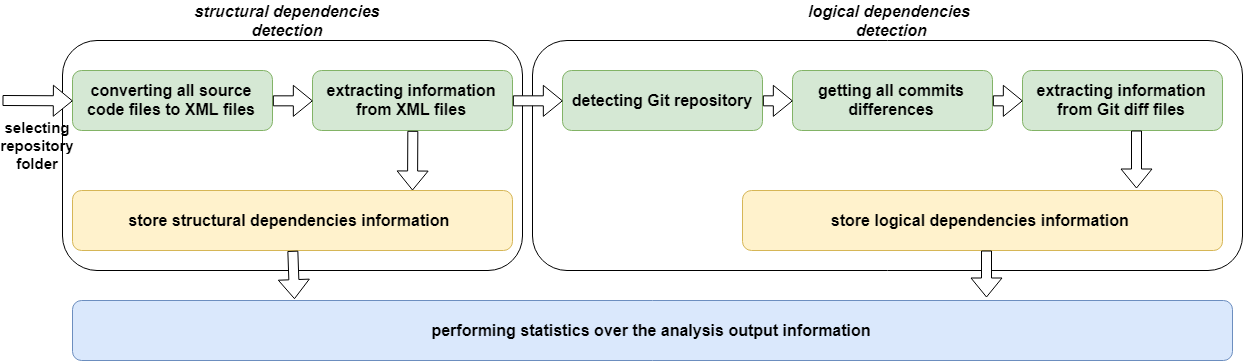
\includegraphics[width=\textwidth]{fig3.png}
\caption{Processing phases}
\label{fig:fig3}
\end{figure*}

\subsection{ Extracting structural dependencies}

%Even though in some of the cases if class A depends on class B, changes in class B can produce changes in class A, but not the other way around \cite{Yu2007}. There are some cases in which if class A depends on class B,  changes in class B can produce changes in class A and viceversa. So we will consider structural dependencies as bidirectional relationships, "class A depends on class B" and "class B depends on class A". The choice of building bidirectional relationships is also motivated by the fact that we cannot establish for the moment the direction of the logical dependencies of the system. So in order to have a omogenity between the logical and structural dependencies analysis results, we will take both of the relationships types as bidirectional.
A structural dependency between two classes A and B is given by the fact that A statically depends on B, meaning that A cannot be compiled without knowing about B. In object oriented system, this dependency can be given by many types of relationships between the two classes: A extends B, A implements B, A has attributes of type B, A has methods which have type B in their signature, A uses local variables of type B.


 We use an external tool called srcML \cite{2003:XLC:851042.857028},
\cite{Collard:2011:LTF:2067850.2068011} to convert all source code files from the current release into XMl files. All the information about classes, methods, calls to other classes are afterwards extracted by our tool parsing the XML files and building a dependencies data structure. We have chosen to rely on srcML as a preprocessing tool because it reduces a significant number of syntactic differences from different programming languages and can make easyer the parsing of source code written in different programming languages such as Java, C++ and C\#.    

\subsection{Extracting logical dependencies}

The versioning system contains the long-term change history of every file. Each project change made by an individual at a certain point of time is contained into a commit \cite{svn}. All the commits are stored in the versioning system chronologically and each commit has a parent. The parent commit is the baseline from which development began, the only exception to this rule is the first commit which has no parent. We will take into consideration only \textit{commits that have a parent} since the first commit can include source code files that are already in development (migration from one versioning system to another) and this can introduce redundant logical links \cite{DBLP:journals/jss/AjienkaC17}. 

The tool looks through the main branch of the project and gets all the existing commits. For each commit a diff against the parent will be made and stored. Here we have the option to ignore commits that contain more files than a threshold value for commit size. Also, we have the option to check whether the differences are in actual code or if they affect only parts of source files that are only comments.  Finally after all the difference files are stored, all the files are parsed and logical dependencies are build. For a group of files that are committed together, logical dependencies are added between all pairs formed by members of the group. Adding a logical dependency increases an occurrence counter for the logical link. 

\section{Experimental results}
\label{sec:experiments}


We have analysed a set of open-source projects found on GitHub\footnote{http://github.com/} in order to extract the structural and logical dependencies between classes. Table \ref{table:1} enumerates all the systems studied. The 1st column assigns the projects IDs; 2nd column shows the project name; 3rd column shows the number of classes extracted; 4th column shows the number of most recent commits analysed from the active branch of each project and the 5th shows the language in which the project was developed.

\begin{table}[h]
	\caption{Summary of open source projects studied.}
	\centering
  \begin{tabular}{@{}ccccc@{}}
    \toprule
    ID  & Project    & Nr. of classes & Nr. of commits& Type\\
    \midrule
 \ch{1}	&	urSQL	&	39	&	89	&	java	\\
 \ch{2}	&	prettyfaces	&	257	&	207	&	java	\\
 \ch{3}	&	jbal	&	102	&	113	&	java	\\
\ch{4}	&	guavatools	&	209	&	85	&	java	\\
\ch{5}	&	monome-pages	&	196	&	280	&	java	\\
\ch{6}	&	kryo	&	289	&	743	&	java	\\
\ch{7}	&	selma	&	267	&	368	&	java	\\
\ch{8}	&	bluecove	&	386	&	1679	&	java	\\
\ch{9}	&	aima-java	&	818	&	1181	&	java	\\
\ch{10}	&	powermock	&	803	&	1512	&	java	\\
\ch{11}	&	restfb	&	713	&	1545	&	java	\\
\ch{12}	&	rxjava	&	2251	&	2468	&	java	\\
\ch{13}	&	metro-jax-ws	&	365	&	2222	&	java	\\
\ch{14}	&	mockito	&	1121	&	1572	&	java	\\
\ch{15}	&	grizzly	&	1170	&	3122	&	java	\\
\ch{16}	&	shipkit	&	222	&	1483	&	java	\\
\ch{17}	&	Tensorflow	&	1104	&	2386	&	cpp	\\

    \bottomrule
  \end{tabular}
  
   \label{table:1}
\end{table}


For each system, we extracted its structural dependencies, its logical dependencies and determined the overlap between the two dependencies sets, in various experimental conditions. 

One variable experimental condition is whether changes in comments only count as logical dependencies. This condition distinguishes between two different cases: 
\begin{itemize}
	\item with comments: a change in source code files is counted towards a logical dependency, even if the change is inside comments only in all files
	\item without comments: commits that changed source code files only by editing comments are ignored as logical dependencies
\end{itemize}

In all cases, we varied the following threshold values: 
 \begin{itemize}
	\item commit size ($cs$): the maximum number of files allowed in a commit to be counted as logical dependency. The values for this threshold were 5, 10, 20 and no threshold (infinity).  
	\item number of occurrences ($occ$): the minimum number of repeated occurrences for a co-change to be counted as logical dependency. The values for this threshold were 1, 2, 3 and 4.  
\end{itemize}

The six tables below present the synthesis of our experiments. 
We have computed the following  values:
\begin{itemize}
	\item the mean ratio of the number of logical dependencies  (LD) to the number of structural dependencies (SD)
   \item the mean percentage of structural dependencies that are also logical dependencies (calculated from the number of overlaps divided to the number of structural dependencies)	
		\item the mean percentage of logical dependencies that are also structural dependencies (calculated from the number of overlaps divided to the number of logical dependencies)
\end{itemize}

In all the six tables, \ref{tab:ratio:comm}, \ref{tab:ratio:nocomm}, \ref{tab:percSD:comm}, \ref{tab:percSD:nocomm},
\ref{tab:percLD:comm}, \ref{tab:percLD:nocomm} we have on columns the values used for the commit size $cs$, while on rows we have the values for the number of occurrences threshold $occ$. The tables contain median values obtained for experiments done under all combinations of the two threshold values, on all test systems. In all tables, the upper right corner corresponds to the most relaxed conditions, while the lower left corner corresponds to the most restrictive conditions.


\begin{table}[!h]
%% increase table row spacing, adjust to taste
\renewcommand{\arraystretch}{1.25}
\caption{Ratio OF number of LD to number of SD, case with comments}
\label{tab:ratio:comm}
\centering

\begin{tabular}{|c|c|c|c|c|}
\hline
	      &	$cs\leq 5$	&	$cs\leq 10$	&	$cs\leq 20$	&	$cs<\infty$	\\
\hline
$occ\geq 1$	&	1.13	&	3.13	&	5.54	&	72.96	\\
$occ\geq 2$	&	0.31	&	1.04	&	1.70	&	26.13	\\
$occ\geq 3$	&	0.11	&	0.44	&	0.80	&	11.84	\\
$occ\geq 4$	&	0.04	&	0.13	&	0.31	&	5.22	\\
\hline
\end{tabular}
\end{table}


\begin{table}[!h]
%% increase table row spacing, adjust to taste
\renewcommand{\arraystretch}{1.25}
\caption{Ratio OF number of LD to number of SD, case without comments}
\label{tab:ratio:nocomm}
\centering

\begin{tabular}{|c|c|c|c|c|}
\hline
	      &	$cs\leq 5$	&	$cs\leq 10$	&	$cs\leq 20$	&	$cs< \infty$	\\
\hline
$occ\geq 1$	&	0.94	&	2.77	&	4.63	&	66.07	\\
$occ\geq 2$	&	0.27	&	0.83	&	1.46	&	21.10	\\
$occ\geq 3$	&	0.08	&	0.35	&	0.63	&	9.29	\\
$occ\geq 4$	&	0.03	&	0.10	&	0.24	&	3.33	\\
\hline
\end{tabular}
\end{table}


\begin{table}[!h]
%% increase table row spacing, adjust to taste
\renewcommand{\arraystretch}{1.25}
\caption{Percentage of SD that are also LD, case with comments}
\label{tab:percSD:comm}
\centering

\begin{tabular}{|c|c|c|c|c|}
\hline
	      &	$cs\leq 5$	&	$cs\leq 10$	&	$cs\leq 20$	&	$cs< \infty$	\\
\hline
$occ\geq 1$	&	13.77	&	23.27	&	36.04	&	66.48	\\
$occ\geq 2$	&	4.11	&	9.90	&	15.79	&	42.05	\\
$occ\geq 3$	&	1.92	&	5.82	&	8.41	&	21.15	\\
$occ\geq 4$	&	0.85	&	2.68	&	5.80	&	13.46	\\
\hline
\end{tabular}
\end{table}


\begin{table}[!h]
%% increase table row spacing, adjust to taste
\renewcommand{\arraystretch}{1.25}
\caption{Percentage of SD that are also LD, case without comments}
\label{tab:percSD:nocomm}
\centering

\begin{tabular}{|c|c|c|c|c|}
\hline
	      &	$cs\leq 5$	&	$cs\leq 10$	&	$cs\leq 20$	&	$cs< \infty$	\\
\hline
$occ\geq 1$	&	13.77	&	22.15	&	34.38	&	63.96	\\
$occ\geq 2$	&	3.67	&	9.17	&	12.53	&	34.62	\\
$occ\geq 3$	&	1.82	&	4.03	&	6.83	&	17.60	\\
$occ\geq 4$	&	0.67	&	2.34	&	4.47	&	11.60	\\
\hline
\end{tabular}
\end{table}


\begin{table}[!h]
%% increase table row spacing, adjust to taste
\renewcommand{\arraystretch}{1.25}
\caption{Percentage of LD that are also SD, case with comments}
\label{tab:percLD:comm}
\centering

\begin{tabular}{|c|c|c|c|c|}
\hline
	      &	$cs\leq 5$	&	$cs\leq 10$	&	$cs\leq 20$	&	$cs< \infty$	\\
\hline
$occ\geq 1$	&	9.40	&	7.81	&	5.53	&	0.89	\\
$occ\geq 2$	&	20.97	&	16.50	&	7.41	&	1.97	\\
$occ\geq 3$&	18.82	&	18.53	&	13.73	&	2.10	\\
$occ\geq 4$&	27.39	&	21.59	&	18.60	&	2.88	\\

\hline
\end{tabular}
\end{table}


\begin{table}[!h]
%% increase table row spacing, adjust to taste
\renewcommand{\arraystretch}{1.25}
\caption{Percentage of LD that are also SD, case without comments}
\label{tab:percLD:nocomm}
\centering
\begin{tabular}{|c|c|c|c|c|}
\hline
	      &	$cs\leq 5$	&	$cs\leq 10$	&	$cs\leq 20$	&	$cs< \infty$	\\
\hline
$occ\geq 1$	&	8.94	&	8.50	&	6.08	&	0.89	\\
$occ\geq 2$	&	23.00	&	16.21	&	7.25	&	1.96	\\
$occ\geq 3$	&	18.78	&	18.67	&	14.47	&	2.09	\\
$occ\geq 4$	&	25.29	&	19.69	&	16.76	&	4.55	\\

\hline
\end{tabular}
\end{table}





\begin{table}
  \centering
  \caption{Number of logical dependencies, for different threshold values for $cs$, when $occ\geq 1$, case with comments}
	\begin{tabular}{@{}cccccc@{}}
    \toprule
		 ID  & SD & LD	&	LD	&	LD	&	LD \\
      &   & $cs\leq 5$	&	$cs\leq 10$	&	$cs\leq 20$	&	$cs< \infty$ \\
    \midrule
 \ch{1}	&	52	&	59	&	145	&	288	&	415	\\
 \ch{2}	&	264	&	21	&	21	&	76	&	76	\\
 \ch{3}	&	106	&	27	&	57	&	231	&	5570	\\
\ch{4}	&	138	&	89	&	210	&	598	&	1023	\\
\ch{5}	&	250	&	239	&	824	&	1593	&	4635	\\
\ch{6}	&	566	&	1576	&	2548	&	4217	&	22437	\\
\ch{7}	&	358	&	223	&	1051	&	1756	&	6845	\\
\ch{8}	&	447	&	687	&	1421	&	2308	&	32612	\\
\ch{9}	&	1463	&	1063	&	2640	&	6257	&	156710	\\
\ch{10}	&	466	&	1052	&	2693	&	5696	&	42726	\\
\ch{11}	&	832	&	1529	&	2604	&	4184	&	32133	\\
\ch{12}	&	2557	&	1172	&	3575	&	9319	&	577118	\\
\ch{13}	&	154	&	488	&	940	&	1811	&	55837	\\
\ch{14}	&	541	&	2360	&	5871	&	9689	&	182276	\\
\ch{15}	&	2698	&	2620	&	6773	&	16058	&	218476	\\
\ch{16}	&	138	&	1519	&	3584	&	6233	&	22145	\\
\ch{17}	&	293	&	1569	&	3253	&	5667	&	32347	\\
\midrule
Median for LD/SD	&	&	1.13	&	3.13	&	5.54	&	72.96	\\
    \bottomrule
  \end{tabular}
  
   \label{table:5}
\end{table}



\begin{table}
  \centering
  
	\caption{Number of logical dependencies, for different threshold values for $cs$, when $occ\geq 1$, case without comments}
	\begin{tabular}{@{}cccccc@{}}
    \toprule
		ID  & SD & LD	&	LD	&	LD	&	LD \\
      &   & $cs\leq 5$	&	$cs\leq 10$	&	$cs\leq 20$	&	$cs< \infty$ \\
    \midrule
 \ch{1}	&	52	&	49	&	121	&	257	&	319	\\
 \ch{2}	&	264	&	19	&	19	&	74	&	74	\\
 \ch{3}	&	106	&	27	&	33	&	171	&	5553	\\
\ch{4}	&	138	&	84	&	194	&	566	&	991	\\
\ch{5}	&	250	&	217	&	712	&	1327	&	4004	\\
\ch{6}	&	566	&	1488	&	2307	&	3928	&	20396	\\
\ch{7}	&	358	&	200	&	918	&	1502	&	4751	\\
\ch{8}	&	447	&	619	&	1255	&	2066	&	31879	\\
\ch{9}	&	1463	&	963	&	2374	&	5632	&	149531	\\
\ch{10}	&	466	&	932	&	2399	&	4729	&	35846	\\
\ch{11}	&	832	&	1373	&	2305	&	3618	&	28401	\\
\ch{12}	&	2557	&	1107	&	3340	&	7948	&	333585	\\
\ch{13}	&	154	&	417	&	758	&	1407	&	51894	\\
\ch{14}	&	541	&	2246	&	5424	&	8504	&	148053	\\
\ch{15}	&	2698	&	2341	&	5716	&	12486	&	178262	\\
\ch{16}	&	138	&	1406	&	3161	&	5475	&	20215	\\
\ch{17}	&	293	&	1539	&	3195	&	5578	&	29720	\\
\midrule
Median for LD/SD	&	&	0.94	&	2.77	&	4.63	&	66.07\\
    \bottomrule
  \end{tabular}
  
   \label{table:6}
\end{table}





\section{Discussion}
\label{sec:discussion}


This section uses the experimental results to answer the research questions outlined in section \ref{sec:question}.

\textit{\textbf{Question 1}}. How does the maximum number of source files accepted to change in a commit influence the logical dependencies of the system ?

Based on the results presented in tables \ref{tab:ratio:comm} and \ref{tab:ratio:nocomm}, the number 
of changed files taken into consideration has an important influence over the ratio of the number  of 
logical dependencies to the number of structural dependencies.  If no threshold is set for the number of files in a commit (the cases in the last column in tables \ref{tab:ratio:comm} and 
\ref{tab:ratio:nocomm} ) then the number of logical dependencies outnumbers the structural dependencies with a factor of up to 73. The maximum factor is measured in the case when no filtering is done on the number of occurrences (first row).  
In this case, we can not talk about logical dependencies, but about classes that happened to once change in the same time, by various reasons. Tables \ref{table:5} and \ref{table:6}  present the detailed situation of the number of logical dependencies, under the conditions of a varying threshold for the number of files accepted in a commit, without any filtering according to the number of occurrences, for all test systems. These tables detail the situations summarized in the 1st rows of tables \ref{tab:ratio:comm} and respectively \ref{tab:ratio:nocomm}. 

When filtering is done according to conditions on the number of occurrences, we observe in tables \ref{tab:ratio:comm} and \ref{tab:ratio:nocomm} that the values on the last column still do not fall below 3.33. This number is still too big to accept for logical dependencies.  It is clear that it is necessary to  put a threshold on the number of files accepted in a commit in order to filter out noise.


If we refer to the overlap between structural and logical dependencies, we can see in tables \ref{tab:percSD:comm} and \ref{tab:percSD:nocomm} that the percentage of structural dependencies which are also logical dependencies is as well affected by setting a threshold on the number of files accepted in a commit. When setting a threshold, then we have less logical dependencies overall and one could say that this is what affects also the smaller number of structural dependencies that are also logical dependencies. However, we can see that the percentage of dependencies in the overlap decreases much slower than the total number of logical dependencies. For example, when setting  the $cs$ threshold at 10, the total number of logical dependencies decreases approx 20 times compared with no threshold, while the overlap decreases less, only approx 3 times. This confirms the fact that the logical dependencies filtered out were not true dependencies. It is clear that setting a threshold on the maximum number of files accepted in a commit is essential for the quality of finding true logical dependencies.


\textit{\textbf{Question 2}}. Considering changes only in comments as valid can lead to additional logical dependencies? How many logical dependencies are introduced by considering comment changes as valid changes and in what percentage this can influence the analysis?

In order to assess the influence of comments, we compare pairwise tables \ref{tab:ratio:comm} and \ref{tab:ratio:nocomm},  
tables \ref{tab:percSD:comm} and \ref{tab:percSD:nocomm} and tables \ref{tab:percLD:comm} and \ref{tab:percLD:nocomm}. 
We observe that, although there are some differences between pairs of measurements done in similar conditions with and without comments, the differences are not significant.

In the case of the ratio of the number of logical dependencies to the number of structural dependencies, from tables \ref{tab:ratio:comm} and \ref{tab:ratio:nocomm} we can see that the maximum difference is for the values from the position of the first row, last column. Without comments, the value of the ratio is 66.07, compared to the value with comments which is 72.96. The decrease represents 10\% of the value with comments. In the case of the percentage of structural dependencies that are also logical dependencies, from tables \ref{tab:percSD:comm} and \ref{tab:percSD:nocomm}, we can see that the maximum difference is also for the values from the first row, last column. Without comments, the overlap is 63.96, compared to the value with comments which is 66.48.  The decrease represents 4\% of the value with comments. We notice that the decrease percentage is smaller for the overlap than for the ratio of the total number of logical dependencies, thus we can say that eliminating changes due only to comments can slightly improve the quality of finding logical dependencies. 



\textit{\textbf{Question 3}}. How many occurrences of a logical dependency are needed to consider it a \textit{valid} logical dependency ? 

If we look at consecutive rows in table \ref{tab:ratio:comm} or in table \ref{tab:ratio:nocomm}, corresponding to increased threshold values for the number of occurrences, we can roughly say that  increasing by 1 the occurrence threshold while maintaining the other conditions reduces with more than half the total number of logical dependencies.  

In order to find the appropriate level of filtering out false logical dependencies, we assume as a rule of thumb that the number of logical dependencies should be not bigger that the number of structural dependencies. On the other hand, choosing the most restrictive combination of thresholds (a commit size threshold of 5 files combined with an occurrence threshold of 4) leads to a very small number of logical dependencies, representing a fraction of only 0.03 from the number of structural dependencies. 
In tables \ref{tab:ratio:comm} or \ref{tab:ratio:nocomm}, we can see that we can obtain a number of logical dependencies which is between one quarter and one third of the number of the structural dependencies either by setting a commit size threshold of 5 files combined with an occurrence threshold of 2, or a commit size threshold of 10 files combined with an occurrence threshold of 3, or a commit size threshold of 20 files combined with an occurrence threshold of 4.  It is clear that increasing the threshold value for number of occurrences can be done only together with increasing the threshold value for maximum number of committed files. A more complex filtering condition can aggregate the 3 simple filtering cases, in the form: $((cs\leq 5) and (occ\geq 2)) or ((cs\leq 10) and (occ\geq 3)) or ((cs\leq 20) and (occ\geq 4))$. In this condition, $occ$ refers actually to 3 different counters, because every filtering on a different $cs$ has its own counter.  


\textit{\textbf{Question 4}}. How does filtering affect the overlap between structural and logical dependencies ? 

In order to present overlaps between structural and logical dependencies we will use Venn diagrams, used for this purpose also in \cite{Oliva:2011:ISL:2067853.2068086} and \cite{DBLP:journals/jss/AjienkaC17}. In Figure \ref{fig_venn} we present the intersections of logical and structural dependencies, in a selection of relevant cases. In all cases, the left circle, which is of constant size, represents the set of structural dependencies. The right circle represents the logical dependencies and its area is proportional with the number of logical dependencies. All cases are cases without comments.

In Figure \ref{fig_venn}, case a.) which corresponds to no filtering, the number of logical dependencies is bigger than the number of structural dependencies by a factor of 66. In this case, we also have the biggest percentage of structural dependencies which are also logical (64\%). This case shows that classes with structural dependencies change together more often, but these changes cannot be yet considered logical dependencies.

In Figure \ref{fig_venn}, case b.) corresponding to the highest level of filtering, the number of logical dependencies is only 3 \% from  the number of structural dependencies. In this case, the percentage of structural dependencies which are also logical is small, as well as the percentage of logical dependencies that are also structural.  The percentage of logical dependencies that are also structural is 25\% in this case. The percentage of logical dependencies that are not structural is 75\%, and we consider that they deserve to be considered as additional dependencies. However, we observe that some logical dependencies get lost, especially in the case of smaller systems.

We consider that an optimal level of filtering is given by threshold combinations such as in cases c.), d.) and e.).  In the case d.) the number of logical dependencies represents one third of the number of structural dependencies. The percentage of structural dependencies which are also logical is 4\%,  while the percentage of logical dependencies that are also structural is 18\%. We can see that a percentage of 82\% of logical dependencies do not correspond with  structural dependencies, while 96\% of the structural dependencies are not doubled by logical dependencies. These percentages are statistically similar with the values obtained in \cite{Oliva:2011:ISL:2067853.2068086}: they measured LCOP (Logical Coupling Only Percentage)  and SCOP (Structural Coupling Only Percentage) and obtained 95\% for SCOP and 91\% for LCOP. In \cite{DBLP:journals/jss/AjienkaC17} they  measured CSD (Co-changes Structural Dependencies ratio) and the CLD (Coupled Logical Dependencies ratio) and obtained the values for CSD about 80\% and CLD about 15\%. The value for CLD is statistically similar with our result for the percentage of logical dependencies that are also structural which we measured 18\%. There is still a significant difference between the value for CSD and our percentage of structural dependencies which are also logical. The explanation for this lies in the different manner of determining the logical dependencies: while \cite{DBLP:journals/jss/AjienkaC17} also uses a threshold of 10 for the maximum number of files in a commit, they count all co-changes toward logical dependencies, although they assign them different strengths. Also in case of \cite{DBLP:journals/jss/AjienkaC17}  the total number of logical dependencies is 10 times bigger than the number of structural dependencies, while in our work, in the case under discussion the total number of logical dependencies is 3 times smaller than the number of structural dependencies.  





\begin{figure*}[!t]
\centering
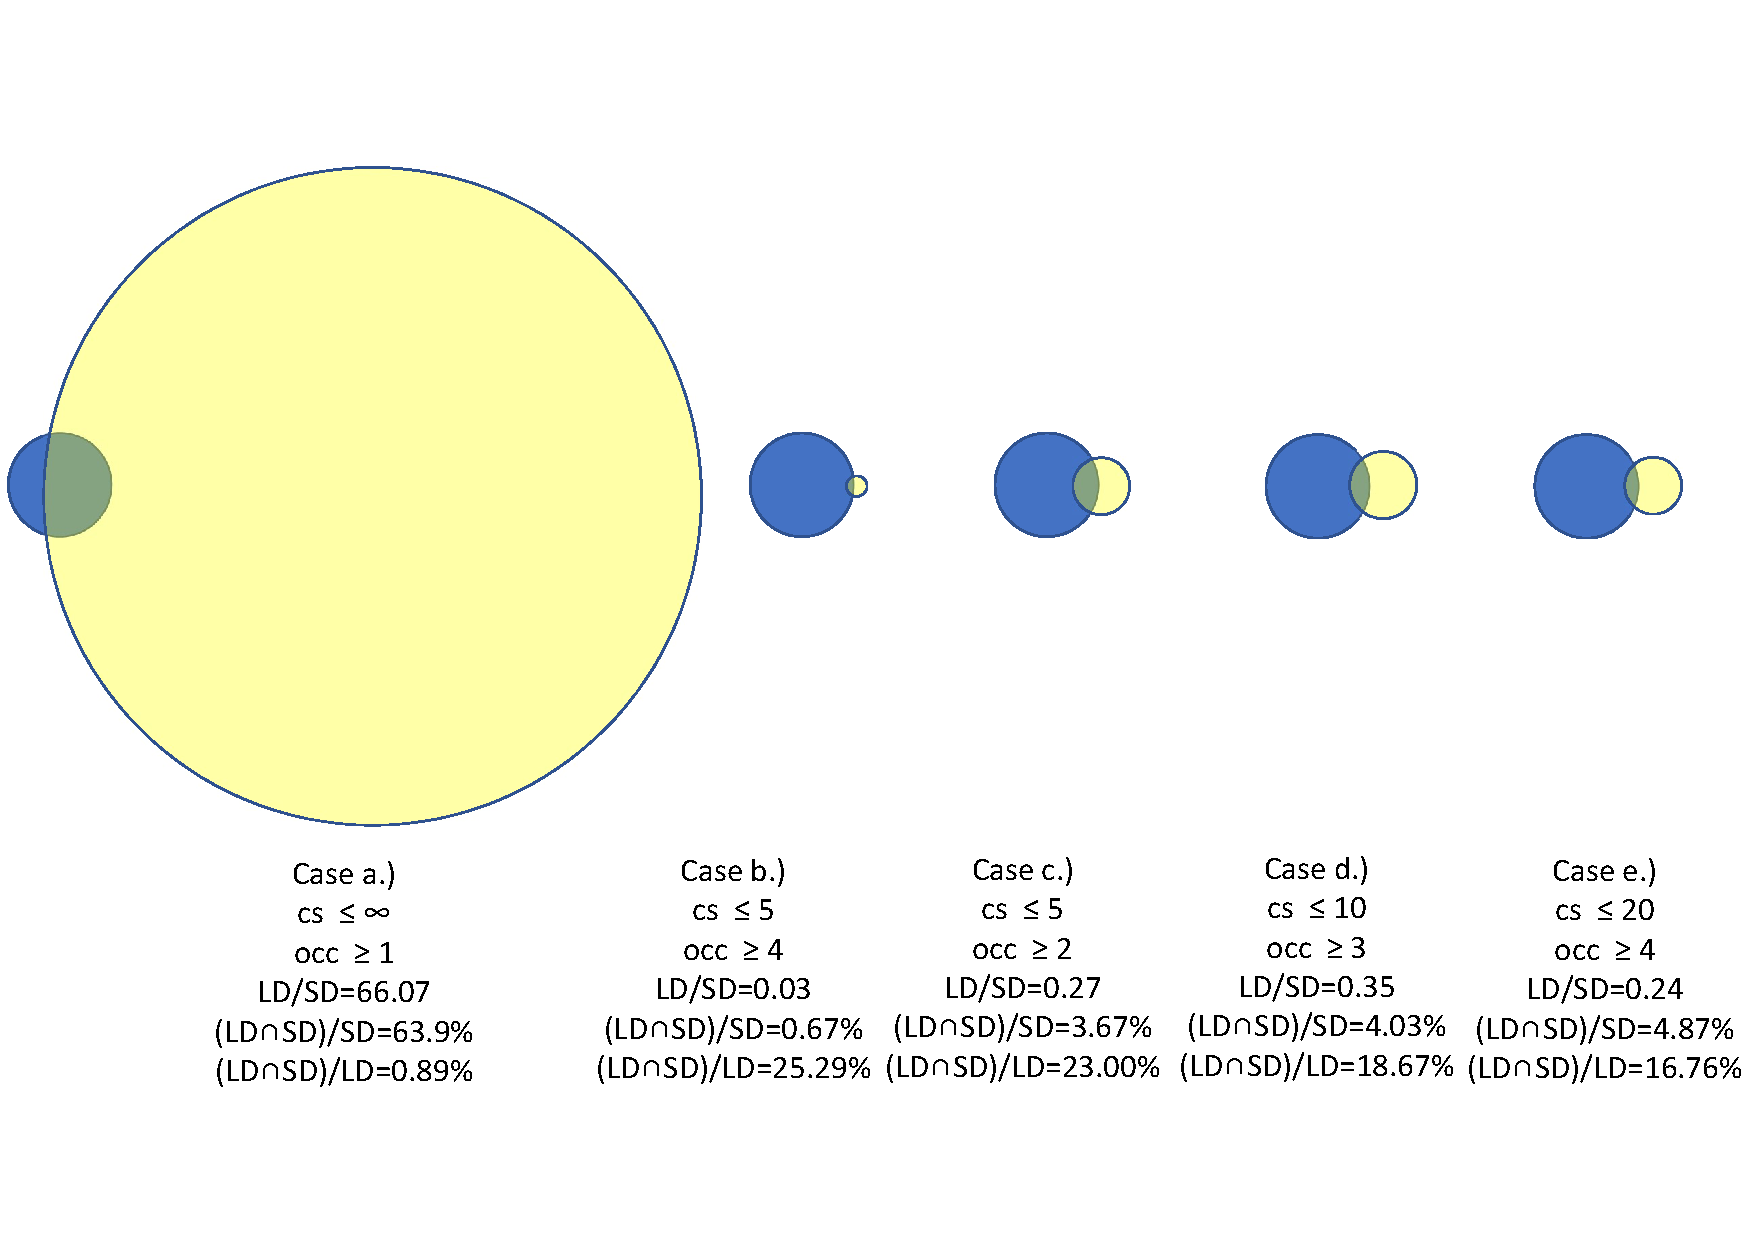
\includegraphics[width=5.7in]{fig.pdf}
\vspace{-1cm}
% where an .eps filename suffix will be assumed under latex, 
% and a .pdf suffix will be assumed for pdflatex; or what has been declared
% via \DeclareGraphicsExtensions.
\caption{Intersections of logical and structural dependencies, in different cases defined by different combinations of filtering thresholds. }
\label{fig_venn}
\end{figure*}




Tables \ref{table:10} and \ref{table:11} relate with table \ref{tab:percSD:comm} and they detail information about overlaps between logical and structural dependencies. Table \ref{table:10} gives details about the cases summarized in the first column, while table \ref{table:11} gives details about the cases summarized in the last column of table \ref{tab:percSD:comm}.
  
\begin{table}[!h]
  \centering
  \caption{Percentage of SD that are also LD,  when $cs \leq 5$, for different threshold values for $occ$ }
	\begin{tabular}{@{}ccccc@{}}
    \toprule
    ID  & $occ\geq 1$ & $occ\geq 2$ & $occ\geq 3$ & $occ\geq 4$  \\
    \midrule
 \ch{1}	&	28.85	&	15.38	&	1.92	&	0.00	\\
 \ch{2}	&	1.89	&	0.76	&	0.38	&	0.38	\\
 \ch{3}	&	1.89	&	0.94	&	0.00	&	0.00	\\
\ch{4}	&	13.77	&	2.17	&	1.45	&	0.72	\\
\ch{5}	&	16.00	&	8.00	&	3.20	&	1.20	\\
\ch{6}	&	22.79	&	12.54	&	4.24	&	2.12	\\
\ch{7}	&	10.34	&	3.63	&	0.56	&	0.28	\\
\ch{8}	&	13.65	&	5.82	&	2.68	&	1.12	\\
\ch{9}	&	6.90	&	1.78	&	0.27	&	0.21	\\
\ch{10}	&	15.67	&	2.58	&	1.07	&	0.86	\\
\ch{11}	&	35.70	&	26.56	&	9.38	&	8.29	\\
\ch{12}	&	1.25	&	0.82	&	0.35	&	0.31	\\
\ch{13}	&	6.49	&	2.60	&	1.30	&	0.00	\\
\ch{14}	&	24.40	&	14.05	&	6.28	&	3.14	\\
\ch{15}	&	12.42	&	4.11	&	2.04	&	0.93	\\
\ch{16}	&	46.38	&	29.71	&	14.49	&	7.97	\\
\ch{17}	&	15.70	&	9.56	&	5.46	&	3.41	\\

\midrule
Median	&	13,77	&	4,11	&	1,92	& 0.85\\	
    \bottomrule
  \end{tabular}
  
   \label{table:10}
\end{table}



\begin{table}[!h]
  \centering
	\caption{Percentage of SD that are also LD,  when  $cs< \infty$, for different threshold values for $occ$ }
  \begin{tabular}{@{}ccccc@{}}
    \toprule
    ID  & $occ\geq 1$ & $occ\geq 2$ & $occ\geq 3$ & $occ\geq 4$ \\
    \midrule
 \ch{1}	&	76.92	&	46.15	&	21.15	&	13.46	\\
 \ch{2}	&	1.89	&	0.76	&	0.38	&	0.38	\\
 \ch{3}	&	85.85	&	84.91	&	83.96	&	81.13	\\
\ch{4}	&	70.29	&	15.22	&	10.87	&	10.14	\\
\ch{5}	&	69.60	&	58.40	&	44.80	&	34.40	\\
\ch{6}	&	65.55	&	42.05	&	30.57	&	21.20	\\
\ch{7}	&	66.48	&	32.68	&	18.99	&	12.57	\\
\ch{8}	&	64.88	&	43.40	&	20.58	&	13.20	\\
\ch{9}	&	75.32	&	58.58	&	41.90	&	23.44	\\
\ch{10}	&	57.73	&	30.69	&	19.53	&	13.30	\\
\ch{11}	&	81.49	&	64.66	&	37.98	&	33.41	\\
\ch{12}	&	14.74	&	8.80	&	5.91	&	3.75	\\
\ch{13}	&	33.12	&	9.74	&	7.79	&	5.84	\\
\ch{14}	&	67.28	&	45.84	&	26.80	&	17.19	\\
\ch{15}	&	52.85	&	33.80	&	22.65	&	15.27	\\
\ch{16}	&	80.43	&	71.01	&	55.07	&	48.55	\\
\ch{17}	&	24.57	&	18.43	&	17.06	&	11.95	\\

\midrule
Median	&	66,48	&	42,04	&	21,15 & 13.46\\		
    \bottomrule
  \end{tabular}
 
   \label{table:11}
\end{table}

Looking at the detailed tables, we can notice that the values for individual projects may present significant differences from the median. For smaller projects, such as projects with IDs 1, 3, 4, the filtering can lead to loosing logical dependencies.  


\section {Threats to validity}
\label{sec:validity}


An issue which has not been investigated enough is whether the reduced set of logical dependencies obtained after filtering contains indeed true logical dependencies. This could be done by manual inspection of the classes in order to validate the reported logical dependencies by the opinion of a human expert. Unfortunately doing such manual validation for all case studies is an impossibly huge task. We have manually inspected the code and code changes from a few of the case studies and the results seem promising. For example, in the case of the project selma, when filtering with both thresholds on commit size and number of occurrences, the tool reduced the initial set of 4751 co-change links identified between classes when no filtering was done, to a number of just 25 logical dependencies. Out of these 25 logical dependencies, 5 are doubled by structural dependencies. From the 20 remaining logical dependencies identified by the tool, we determined by manual inspection that 18 are logical, while for 2 of them we could not see a logical reason for a dependency relationship. 
%The 18 class pairs where we could confirm by manual inspection a logical link are: ('FieldItem', 'MapperMethodGenerator'),  ('CollectionsMapperIT', 'MappingBuilder'), ('MapperMethodGenerator', 'MethodWrapper'), ('MapperMethodGenerator', 'MappingSourceNode'),  ('MapperMethodGenerator', 'MappingBuilder'), ('MapperMethodGenerator', 'BeanWrapper'), ('MapperMethodGenerator', 'InOutType'), ('MapperMethodGenerator', 'FailingMappersIT'),  ('MapperMethodGenerator', 'FailingMissingPropertyMapsMappersIT'), ('MapperMethodGenerator', 'MapperWrapper'), ('MapperMethodGenerator', 'MappingRegistry'),  ('CustomMapperWrapper', 'FactoryWrapper'),  ('CustomMapperWrapper', 'MappingBuilder'),  ('CustomMapperWrapper', 'MapperClassGenerator'), ('MappingRegistry', 'MapperClassGenerator'), ('InOutType', 'MappingBuilder'),  ('MappingBuilder', 'MappingSourceNode'),  ('FactoryWrapper', 'MapperClassGenerator').

We consider that in the future, the validation of extracted logical dependencies will occur by using them to enhance dependency graphs for  applications such as architectural reconstruction through clustering \cite{SoraConti} or finding of key classes \cite{PagerankENASE}, and evaluating the positive impact on their results.   


As we could see in tables \ref{tab:percLD:comm} and \ref{tab:percLD:nocomm}, only a small amount of logical dependencies are between classes that also present structural dependencies.  In our experiments, even after filtering, around 80\% of the logical dependencies are between classes without structural dependencies. Although this big percentage is supported also by experiments of related works, we consider that future work must further investigate its cause. One possible cause could be that some of the co-changes were legit logical dependencies at some moment in the past, maybe even doubled by structural dependencies in previous revisions, but in the mean time the problem causing them may have been refactored and they should not be added to the dependency model of the current system.  

In this work we have extracted logical dependencies from all the revisions of the system, and structural dependencies from the last revision of the system. In future work we will take into account also structural dependencies from all the revisions of the system, in order to filter out the old, out-of-date logical dependencies.  Some logical dependencies may have been also structural in previous revisions of the system but not in the current one. If we take into consideration also structural dependencies from previous revisions then the overlapping rate between logical and structural dependencies could probably increase. Another way to investigate this problem could be to study the trend of occurrencies of co-changes: if co-changes between a pair of classes used to happen more often in the remote past than in the more recent past, it may be a sign that the problem causing the logical coupling has been removed in the mean time. 


   


\section{Conclusion}
\label{sec:Conclusion}
   
In this work we experimentally define methods to filter out the most relevant logical dependencies from co-changing classes. 

Regarding whether co-changes which affect only comments contribute to logical dependencies, our study has found out that when ignoring commits which change only comments in source files, the quality of logical dependencies is slightly improved.

Our experiments show that the most important factors which affect the quality of logical dependencies are: the maximum number of files allowed in a commit to be counted as logical dependency, and the minimum number of repeated occurrences for a co-change to be counted as logical dependency. An important conclusion is that increasing the threshold value for the number of occurrences can be done only together with increasing the threshold value for the maximum number of files allowed in a commit.

 
\bibliographystyle{apalike}
{\small
\bibliography{logicaldepd}}
 

\end{document}

